\documentclass[11pt]{scrreprt}
\usepackage[utf8]{inputenc}

\usepackage[T1]{fontenc}
\usepackage{helvet}
\renewcommand{\familydefault}{\sfdefault}
\addtokomafont{chapter}{\LARGE}
\renewcommand*{\chapterformat}{\thechapter\hspace{0.4cm}}
\RedeclareSectionCommand[style=section]{chapter}

\usepackage{graphicx}
\usepackage[export]{adjustbox}
\usepackage{sectsty}
\usepackage{titlesec}
\usepackage{url}
\usepackage{hyperref}
\usepackage{svg}

\usepackage{minted}
\usemintedstyle{borland}
\definecolor{bg}{rgb}{0.85,0.85,0.85}
\setminted{linenos=true,fontsize=\small,bgcolor=bg}

% Margins
\topmargin=-0.45in
\evensidemargin=0in
\oddsidemargin=0in
\textwidth=6.5in
\textheight=9.0in
\headsep=0.25in


\begin{document}

\begin{titlepage}
    \centering
    \vspace{4\baselineskip}
    Instituto Tecnológico y de Estudios Superiores de Monterrey\par
    Campus Monterrey\par
    \vspace{2\baselineskip}
    {\large
    TC-3048 Compiler design}\par
    \vspace{6\baselineskip}
    {\huge
    miniclj\par}
    {\LARGE
    Design document\par}
    \vspace{4\baselineskip}
    {\Large
    Mario Emilio Jiménez Vizcaíno\\ A01173359\par}
    \begin{figure}[H]
      \centering
      \includegraphics[width=100pt]{firma.png}
    \end{figure}
    \vfill
    Elda Guadalupe Quiroga\par
    Héctor Gibrán Ceballos\par
    \vspace{4\baselineskip}
    November 24th, 2021
\end{titlepage}

\pagebreak

\tableofcontents

\pagebreak

\chapter{About the project}
\section{Project scope}
This project's aim is to create a compiler and virtual machine for a lisp-based language with similar semantics to Clojure. The base functions and data structures will be supported, and they must be accessible either through a Command-Line Interface or inside a web context.

\section{Requirements}
\begin{enumerate}
  \item The compiler must be able to parse and recognize s-expressions.
  \item The compiler must include a specific syntax for creating inline data structures such as lists, vectors, maps and sets
  \item The compiler must check for lexic, syntax and semantic errors, and display an appropiate error message in these cases
  \item The compiler must emit bytecode similar to quadruples, translating symbols to memory addresses, and the tree-based structure of s-expressions to a list of instructions
  \item The virtual machine must be able to execute the bytecode produced by the compiler
  \item The virtual machine must check semantic errors that couldn't be checked during compilation, such as the arity of callables and user defined functions
  \item Both the compiler and virtual machine must use data structures that enable them to do their job efficiently and without wasting memory
\end{enumerate}

Some test cases for these requirements can be found in \hyperref[examples]{section \ref{examples}: Code examples}.

\section{Development process}
The development of the language can be tracked from its \href{https://github.com/MarioJim/miniclj}{GitHub repository: MarioJim/miniclj}. The list of commits since the last time this document was generated can also be found in appendix \ref{apdx:commits}.

\subsection{Weekly logs}
During the development I've also kept a weekly log in Spanish of my progress. It can be found in the README.md file in the root directory, or in appendix \ref{apdx:weeklylogs}.

\subsection{Final thoughts}
I would say that this project has helped me learn more about how complex compilers are, because, even though the compiler I wrote is reasonably simple, I've had to build strong abstractions over many of the simple functions of my language, and making sure my abstractions work correctly during compilation and execution has been the hardest challenge I've encountered in this project.
\begin{figure}[H]
  \includegraphics[width=100pt,right]{firma.png}
\end{figure}


\chapter{About the language}
\section{Language name}
I chose the name \texttt{miniclj} because this project aims to be a Clojure clone, with a subset of the language's functionality. The syntax and expressions are similar to Clojure's, but some special commands and data structures aren't available, such as support for macros (\texttt{defmacro}), symbols (also known as identifiers, they are replaced during compilation) and concurrency primitives (atoms, \texttt{swap!}, promises, \texttt{deliver}).

\section{Language features}
\texttt{miniclj} offers the basic functionality of a lisp-based language, such as a language based on s-expressions and first-class support for lists and lambda functions. Other features inherited from Clojure are more collection types (vectors, sets and maps) and support for strings as lists of characters. For more information check out the User Manual.

An online version of the language can be found in \href{https://mariojim.github.io/miniclj/}{\texttt{miniclj}'s playground at mariojim.github.io/miniclj/}.

\section{Errors}
The errors for each compilation and execution stage are the following:

\subsection{Parser errors}
This errors are the ones implemented by \texttt{lalrpop}, the parser generator library the language uses, and they are variants of the \href{https://github.com/lalrpop/lalrpop/blob/fc9986c725d908a60b11d8480711afa33f7f3564/lalrpop-util/src/lib.rs#L15}{enum \texttt{ParseError}, found in the file src/lib.rs from the lalrpop-util crate}.
\begin{itemize}
  \item \texttt{InvalidToken}: Returned when the parser encounters a token that isn't part of the language's grammar
  \item \texttt{UnrecognizedEOF}: Returned by the parser when it encounters an EOF it did not expect
  \item \texttt{UnrecognizedToken}: Returned when the parser encounters a token it didn't expect in that position
  \item \texttt{ExtraToken}: Returned when the parser encounters an additional, repeated token
  \item \texttt{User}: Returned by the parser when a custom validation doesn't pass. This type of error is can only be returned while parsing bytecode from its string representation during execution, when a language function isn't recognized or when a memory address couldn't be parsed correctly.
\end{itemize}

\pagebreak
\subsection{Compiler errors}
This errors are implemented as variants of the \texttt{CompilationError} enum, file \path{miniclj-lib/src/compiler/error.rs}.

\inputminted[firstline=9,lastline=35]{rust}{/home/mario/git/MarioJim/miniclj/miniclj-lib/src/compiler/error.rs}

\subsection{Runtime errors}
This errors are implemented as variants of the \texttt{RuntimeError} enum, file \path{miniclj-lib/src/vm/error.rs}.

\inputminted[firstline=5,lastline=45]{rust}{/home/mario/git/MarioJim/miniclj/miniclj-lib/src/vm/error.rs}


\chapter{About the compiler}

\section{Tools and libraries}
The compiler is written in Rust, and it has a couple of dependencies:
\begin{itemize}
  \item \texttt{lalrpop}: used as a lexer and parser for the language
  \item \texttt{num}: used for its implementation of a fraction of 64 bit integers, \texttt{Rational64}
  \item \texttt{smol\_str}: this package is used to keep small strings (less than 22 bytes) in the stack instead of allocating them in the heap
\end{itemize}

\section{Tokens}
The language recognizes the following tokens, separated in string literals and regular expressions:

\subsection{String literals}
\begin{itemize}
  \item "\texttt{(}": ParenOpen
  \item "\texttt{\#(}": ShorthandLambdaOpen
  \item "\texttt{'(}": ListOpen
  \item "\texttt{)}": ParenClose
  \item "\texttt{[}": BracketOpen
  \item "\texttt{]}": BracketClose
  \item "\texttt{{}": BracesOpen
  \item "\texttt{\#\{}": SetOpen
  \item "\texttt{}}": BracesClose
  \item "\texttt{nil}": Nil
  \item "\texttt{\%}": ShorthandLambdaArgument
  \item "\texttt{=}": ComparisonOp::Eq
  \item "\texttt{!=}": ComparisonOp::Ne
  \item "\texttt{>}": ComparisonOp::Gt
  \item "\texttt{<}": ComparisonOp::Lt
  \item "\texttt{<=}": ComparisonOp::Ge
  \item "\texttt{>=}": ComparisonOp::Le
  \item "\texttt{+}": FactorOp::Add
  \item "\texttt{-}": FactorOp::Sub
  \item "\texttt{*}": FactorOp::Mul
  \item "\texttt{/}": FactorOp::Div
\end{itemize}

\subsection{Regular expressions}
\begin{itemize}
  \item \texttt{r"[-]?[0-9]+"}: IntegerLiteral
  \item \texttt{r"[-]?[0-9]+.[0-9]+"}: DecimalLiteral
  \item \texttt{r\#""[\^{}"]*""\#}: StringLiteral
  \item \texttt{r"[A-Za-z][A-Za-z0-9!?'\_-]*"}: UserDefinedSymbol
\end{itemize}

\section{Grammar rules}
The grammar of the language is described in the file \path{miniclj-lib/src/parsers/lispparser.lalrpop}, included in appendix \ref{apdx:grammar}. It describes the following rules:
\begin{itemize}
  \item \textbf{SExprs}
  \begin{itemize}
    \item \textbf{SExpr} \textbf{SExprs}
    \item \textbf{SExpr}
  \end{itemize}
  \item \textbf{SExpr}
  \begin{itemize}
    \item ParenOpen \textbf{SExprs} ParenClose
    \item ParenOpen ParenClose
    \item ShorthandLambdaOpen \textbf{SExprs} ParenClose
    \item ListOpen ParenClose
    \item ListOpen \textbf{SExprs} ParenClose
    \item BracketOpen BracketClose
    \item BracketOpen \textbf{SExprs} BracketClose
    \item BracesOpen BracesClose
    \item BracesOpen \textbf{SExprs} BracesClose
    \item SetOpen BracesClose
    \item SetOpen \textbf{SExprs} BracesClose
    \item \textbf{Literal}
  \end{itemize}
  \item \textbf{Literal}
  \begin{itemize}
    \item Nil
    \item \textbf{Symbol}
    \item StringLiteral
    \item \textbf{NumberLiteral}
  \end{itemize}
  \item \textbf{NumberLiteral}
  \begin{itemize}
    \item DecimalLiteral
    \item IntegerLiteral
  \end{itemize}
  \item \textbf{Symbol}
  \begin{itemize}
    \item ShorthandLambdaArgument
    \item \textbf{ComparisonOp}
    \item \textbf{FactorOp}
    \item UserDefinedSymbol
  \end{itemize}
  \item \textbf{ComparisonOp}
  \begin{itemize}
    \item ComparisonOp::Eq
    \item ComparisonOp::Ne
    \item ComparisonOp::Gt
    \item ComparisonOp::Lt
    \item ComparisonOp::Ge
    \item ComparisonOp::Le
  \end{itemize}
  \item \textbf{FactorOp}
  \begin{itemize}
    \item FactorOp::Add
    \item FactorOp::Sub
    \item FactorOp::Mul
    \item FactorOp::Div
  \end{itemize}
\end{itemize}

During parsing, the full source code of the file is read, and then, depending on the s-expressions parsed, the bytecode is generated. There aren't any additional actions executed during parsing.

\section{Syntaxis diagrams}
\begin{figure}[H]
  \centering
  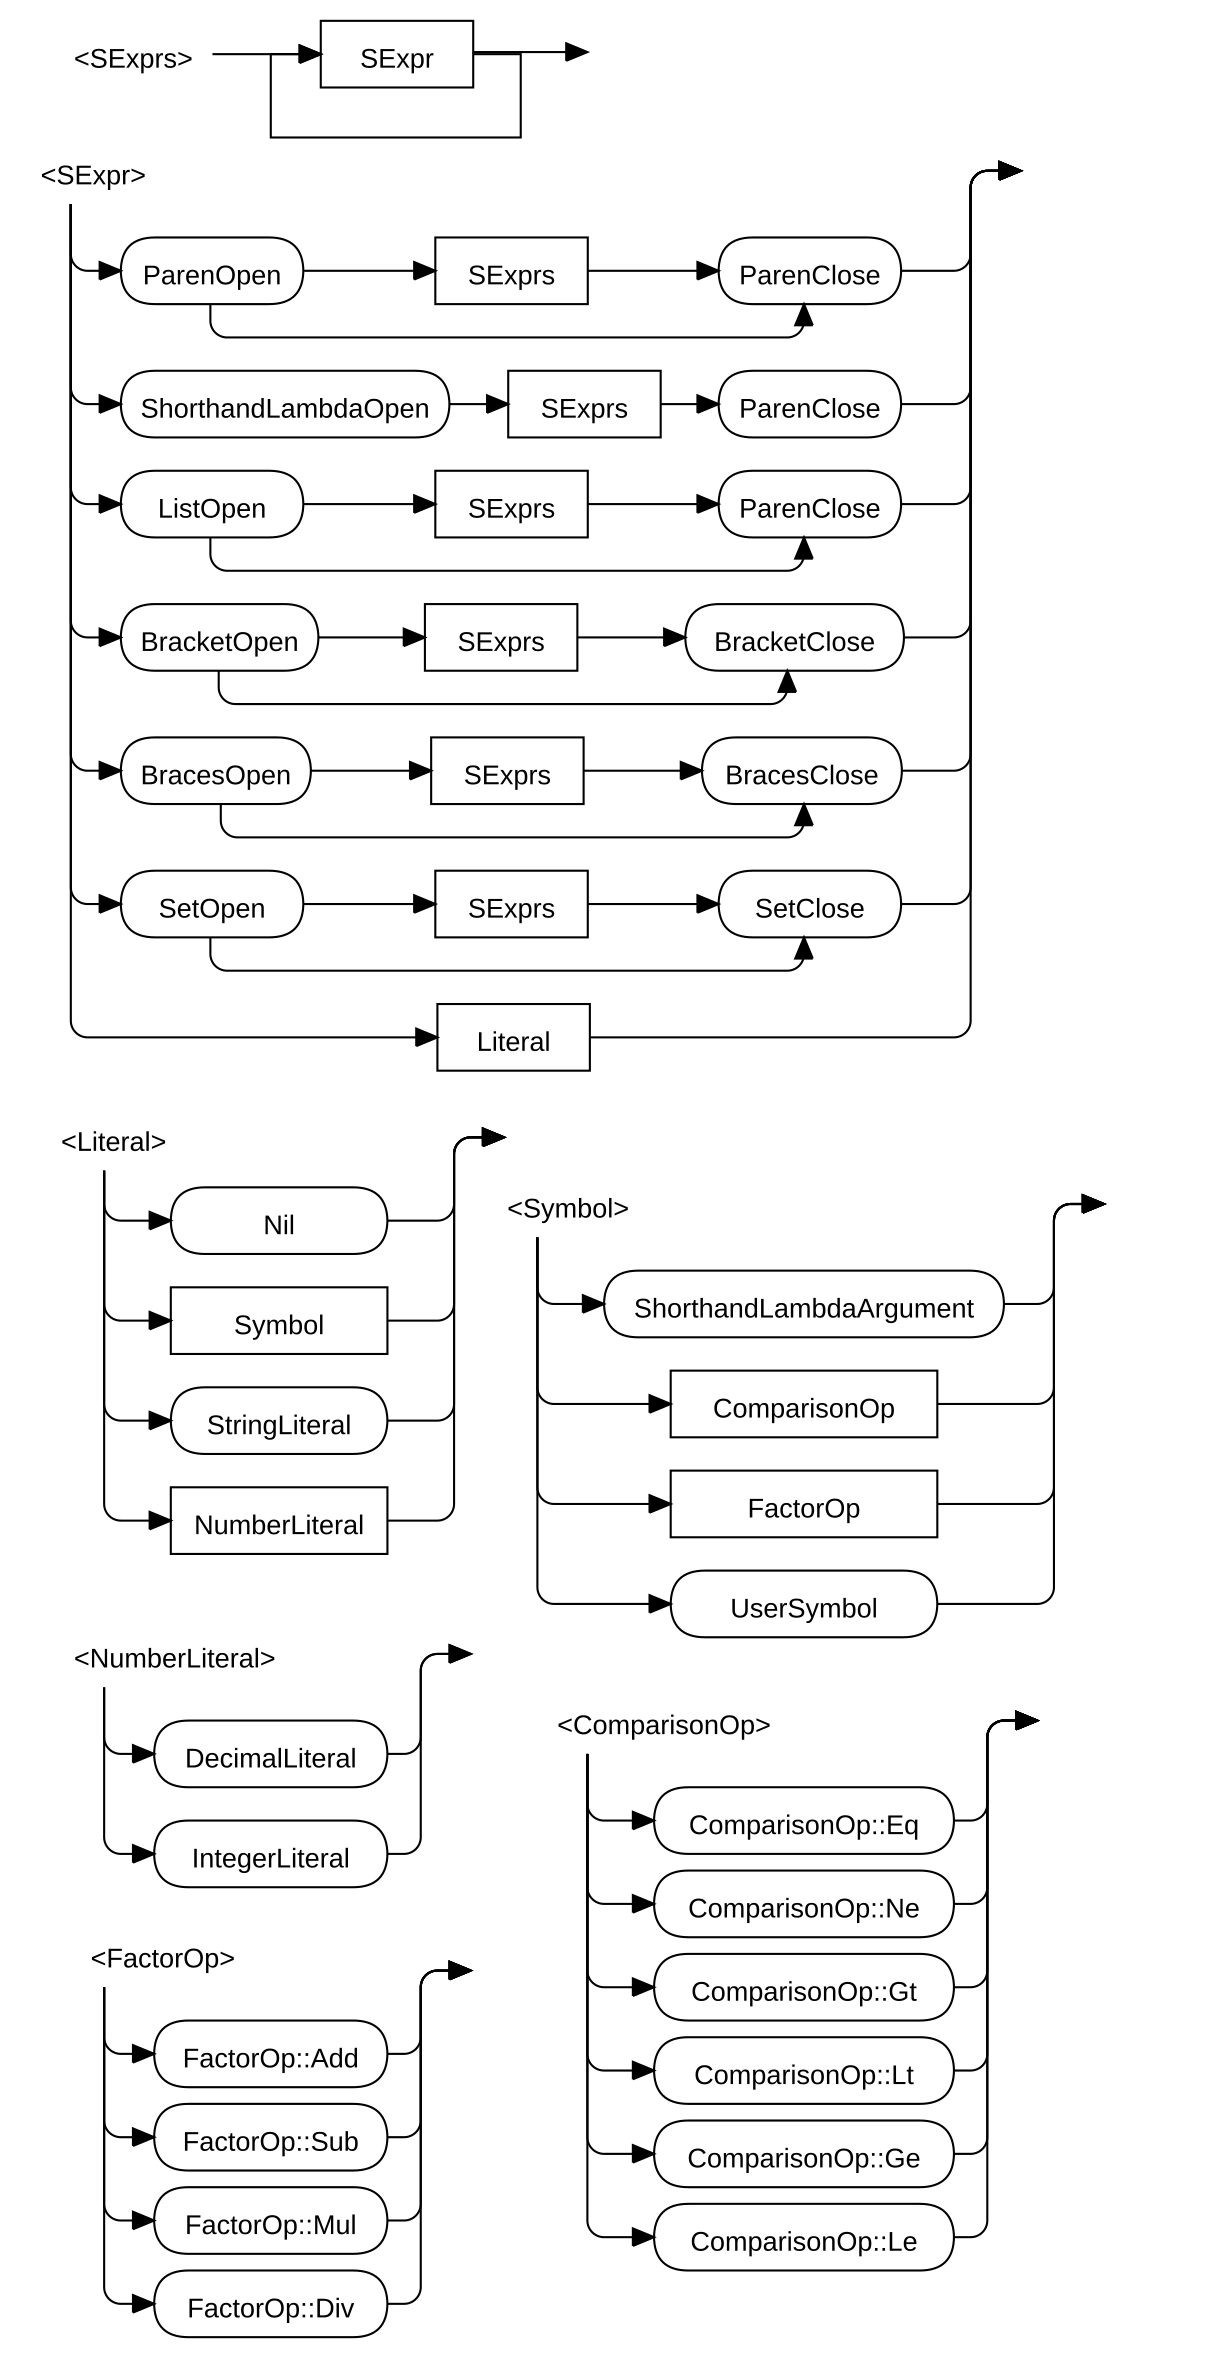
\includegraphics[height=650pt]{SyntaxisDiagrams.png}
\end{figure}


\section{\texttt{CompilerState} struct}
The compiler state is enclosed inside the \texttt{CompilerState} struct, inside file \path{miniclj-lib/src/compiler/state.rs}.

\inputminted[firstline=13,lastline=21]{rust}{/home/mario/git/MarioJim/miniclj/miniclj-lib/src/compiler/state.rs}

This structure is composed of 5 data structures:
\begin{itemize}
  \item \texttt{constants}: This hashmap stores the relationships between the constants and their memory addresses. I decided to use a map instead of a vector so that repeated constants occupy the same address. This map is accessed by the following methods of the \texttt{CompilerState} struct:
  \begin{itemize}
    \item \texttt{insert\_constant}: Receives a constant and returns a memory address. This method has two branches: when the constant was already added to the constants map, this metod just returns a copy of the address assigned to the constant. In case the constant wasn't found in the constants table, the compiler finds the next address available by iterating through the map and inserts the constant with that address.
  \end{itemize}
  \item \texttt{instructions}: This vector stores the list of instructions that will be later executed by the VM. It is accessed by the following methods:
  \begin{itemize}
    \item \texttt{add\_instruction}: Receives an instruction, appends it to the vector, and returns the index of the new instruction
    \item \texttt{instruction\_ptr}: Returns the length of the instructions vector, used as the index of the following instruction to be inserted
    \item \texttt{fill\_jump}: Receives two instruction pointers: the first one is the index of the jump instruction to be modified, and the second one the instruction that it should point to. If the first instruction pointer doesn't refer to a jump instruction, the compiler crashes.
  \end{itemize}
  \item \texttt{symbol\_table}: This custom structure, described in file \texttt{miniclj-lib/src/compiler/\\symboltable.rs} and implemented as a linked list, has three fields:
  \begin{itemize}
    \item \texttt{symbols}: A hashmap of identifiers (declared inside the current scope) to memory addresses
    \item \texttt{temp\_counter}: A counter of how many temporal variables have been created in the current scope
    \item \texttt{var\_counter}: A counter of how many local variables have been assigned in the current scope
  \end{itemize}
  This data structure is accessed by the following methods:
  \begin{itemize}
    \item \texttt{get\_symbol}: Receives a reference to a string and returns either the memory address that points to the value of the identifier or no memory address in case that the symbol couldn't be found in the scope
    \item \texttt{new\_address}: Receives a \texttt{Lifetime} variant to determine if the new address should be a temporal, local or global address, and returns a new memory address
    \item \texttt{insert\_symbol}: Receives a string and an address, and inserts them into the corresponding symbol table (either the current symbol table if the address is local, or the global symbol table if the address has a global lifetime)
    \item \texttt{remove\_symbol}: Receives a reference to a string and removes the symbol from the scope
  \end{itemize}
  \item \texttt{loop\_jumps\_stack}: This structure, although represented as a vector, is used as a stack of pairs of instruction pointers and vectors of memory addresses. This stack is useful for loop/recur cycles, where the compiler has to check where was the last \texttt{loop} instruction declared, so that when a \texttt{recur} instruction is found:
  \begin{enumerate}
    \item The compiler can check that it has the same number of arguments
    \item It can copy the value from each argument to the memory address of the \texttt{loop}'s declaration
    \item It can emit the goto instruction to the \texttt{loop} instruction
  \end{enumerate}
  This process is documented in file \path{miniclj-lib/src/callables/scopefns.rs}, and\\\texttt{CompilerState} exposes the following methods to modify the \texttt{loop\_jumps\_stack}:
  \begin{itemize}
    \item \texttt{push\_loop\_jump}: Receives an instruction pointer and a vector of memory addresses, and appends the pair to the stack
    \item \texttt{pop\_loop\_jump}: Returns a pair of instruction pointer and vector of memory addresses, or nothing if the stack is empty
  \end{itemize}
  \item \texttt{callables\_table}: This custom structure, implemented as a map between strings and structs that implement the \texttt{Callable} trait. It is declared in file \path{miniclj-lib/src/callables/mod.rs}, and it is used to manage the compilation for callables, that consists of:
  \begin{itemize}
    \item For most callables, compile the arguments, add the callable to the constants table and emit an \texttt{Call} instruction for the callable's address, the resulting address of each argument and the temporal address where the result of the call will be stored.
    \item For the other callables, each one may have a different, custom compilation process, like the ones that modify the scope (\texttt{def}, \texttt{defn}, \texttt{let}), the ones used as cycles (\texttt{loop}, \texttt{recur}) and others (like \texttt{fn})
  \end{itemize}
\end{itemize}

This structure also exposes a couple of methods that are use throughout the compilation process:
\begin{itemize}
  \item \texttt{compile}: This is the main method of the compiler: it receives an \texttt{SExpr}, it modifies its state depending on the variant of s-expression that it received, and returns either the resulting memory address of the expression, or a compiler error.
  \item \texttt{compile\_lambda}: This method recieves a list of argument names (of the function that will be compiled) and an \texttt{SExpr} that contains the body of the function
  \item \texttt{write\_to}: This method is used to serialize the compiler state into its string representation, first writing the constants table to the file, and then writing all the instructions in order. More information about this representation can be found in section \ref{comp:bytecode}
  \item \texttt{into\_parts}: Finally, this method is used when the compiler state, instead of being printed to a file, is decomposed to create the state of a VM. It returns the constants and the instructions of the compiler
\end{itemize}

\section{Bytecode representation}
\label{comp:bytecode}
A bytecode file produced by the \texttt{miniclj} compiler, with the extension \texttt{.mclj}, is composed of two parts separated by a line with three asterisks: a list of constant and memory address pairs and a list of instructions. The pairs from the first part are only separated by a space.

\subsection{Constants}
The constants, defined in file \path{miniclj-lib/src/constant.rs}, have 5 different variants:
\begin{itemize}
  \item \texttt{Callable}: Stores a reference to a language callable
  \item \texttt{Lambda}: Has two fields: the instruction pointer that the VM must jump to to execute the lambda, and the number of arguments that the lambda accepts
  \item \texttt{String}: Stores a string literal inside
  \item \texttt{Number}: Stores a \texttt{Rational64} struct inside (\texttt{num}'s implementation of fraction between two signed integers of 64 bits)
  \item \texttt{Nil}: The nil value
\end{itemize}

They are serialized (and deserialized) pretty easily:
\begin{itemize}
  \item \texttt{Callable}: Only the callable name is stored
  \item \texttt{Lambda}: Both numbers are inserted after the string "fn", separated by the at sign (@)
  \item \texttt{String}: The string literal is printed between double quotes
  \item \texttt{Number}: The denominator is printed, then a slash (/) and finally the numerator
  \item \texttt{Nil}: The string "nil" is printed (without quotes)
\end{itemize}

\subsection{Memory addresses}
Memory addresses are composed of two fields:
\begin{itemize}
  \item A \texttt{lifetime} field, of type \texttt{Lifetime}, which specifies the scope of the address. It can be either constant, global, local or temporal.
  \item The index of the address (represented by an unsigned integer)
\end{itemize}

They are serialized as unsigned 32 bit integers, where the first 4 bytes are reserved for the lifetime (constant being $1 * (2 << 28)$, global $2 * (2 << 28)$, and so on), and the other 28 bits are reserved for the index of the variable. The string representation of these addresses is just the number printed as is.

\subsection{Instructions}
The enum \texttt{Instruction} represents the type of instructions that the VM can execute. It has 6 variants and it is declared on the file \path{miniclj-lib/src/instruction.rs}. Here's a short description of each type:
\begin{itemize}
  \item \texttt{Call}: Has 3 fields: the memory address of the callable, the list of memory addresses of the arguments, and the memory address where the result should be stored. This instruction is serialized starting with the string "call", then the address of the callable, the arguments and the result, separated by spaces
  \item \texttt{Return}: This instruction represents the return instruction from a lambda function, and it stores only the memory address of the value that the function will return. It is serialized as the keyword "ret", a space, and then the address
  \item \texttt{Assignment}: This instruction is used to copy a value from an address to another one. It stores the source and destination addresses, and is serialized starting with the keyword "mov", a space, the source address, another space, and the destination address
  \item \texttt{Jump}: This instruction represents an inconditional jump, and it stores only the instruction pointer to which the virtual machine should jump to. It is serialized using the word "jmp", a space, and the instruction pointer
  \item \texttt{JumpOnTrue}: This instruction is used when a jump should only be executed if a value is true. It stores the memory address of the value it should check and the instruction pointer it should jump to, and it is serialized with the keyword "jmpT", a space, the address, another space, and the instruction pointer
  \item \texttt{JumpOnFalse}: This instruction is almost the same as the last one, but only executing the jump if the value referenced by the memory address is false, and with being serialized with the keyword "jmpF"
\end{itemize}


\chapter{About the virtual machine}

\section{Tools and libraries}
The virtual machine, also implemented in Rust, uses the same dependencies as the compiler through the \texttt{num} callable that parses a number from a string, plus the module \texttt{escape8259}, that exports a function used to escape some characters (like \texttt{$\backslash$n} to a newline character) when calling \texttt{print} or \texttt{println}.

\section{\texttt{VMState} struct}
The execution state is stored in the \texttt{VMState} structure, declared in file \path{miniclj-lib/src/vm/state.rs}.

\inputminted[firstline=10,lastline=16]{rust}{/home/mario/git/MarioJim/miniclj/miniclj-lib/src/vm/state.rs}

This structure is composed of 3 fields:
\begin{itemize}
  \item \texttt{constants}: A map of memory addresses to constants, read and constructed from the first part of the bytecode representation
  \item \texttt{instructions}: A vector of instructions, read from the second part of the bytecode file
  \item \texttt{global\_scope}: This field is implemented as a custom structure named \texttt{Scope} (declared in file \path{miniclj-lib/src/vm/scope.rs}, explained in detail in the next section), and it is composed of two vectors of values: one for declared variables and one for temporal values. This structure is used for global and local variables declared in the root scope, and a new \texttt{Scope} is created when executing user defined functions with local variables
\end{itemize}

The main function of the structure \texttt{VMState} is \texttt{execute}, which calls a private method named \texttt{inner\_execute}, implemented as a big match expression (like a switch statement) over the instructions that the virtual machine accepts.

Another important method is \texttt{execute\_lambda} which, as the name implies, executes a lambda function defined by the user. It starts by checking the arity of the function, then creates a new \texttt{Scope}, inserts the local parameters at the start of the scope and also calls \texttt{inner\_execute}.

\section{\texttt{Scope} struct}
As described earlier, memory is represented by the structure \texttt{Scope}, where values are stored inside two vectors.

\inputminted[firstline=7,lastline=13]{rust}{/home/mario/git/MarioJim/miniclj/miniclj-lib/src/vm/scope.rs}

This structure has 4 methods: two \texttt{get} methods for temporal values and variables, which accept an index and return either the value of the vector at that index, or a \texttt{RuntimeError::CompilerError} when the value wasn't found; and two \texttt{store} methods, also for temporal values and variables, which receive an index and a \texttt{Value}, which is then stored in the corresponding vector.

The \texttt{get} methods from \texttt{Scope} are called by a \texttt{get} method in \texttt{VMState}, which receives a reference to the current scope and a memory address, and then routes the request depending on the lifetime of the memory address:
\begin{itemize}
  \item In case that it has a \texttt{Constant} lifetime, this method checks the \texttt{constants} field in \texttt{VMState}
  \item If the address has a \texttt{GlobalVar} lifetime, it checks the \texttt{global\_scope} field also in \texttt{VMState}
  \item If the address has either a \texttt{LocalVar} or \texttt{Temporal} lifetime, the request is routed to the current scope passed to the function
\end{itemize}

The same process happens with the \texttt{store} function in \texttt{Scope}: \texttt{VMState} has a method called \texttt{store} which routes its requests depending on the lifetime of the address, with an exception for \texttt{Constant} addresses, which aren't supposed to be modified during runtime.

This structure is created once to represent the global scope, and then every time a user-defined function is executed, as shown in the diagram.

\begin{figure}[H]
  \centering
  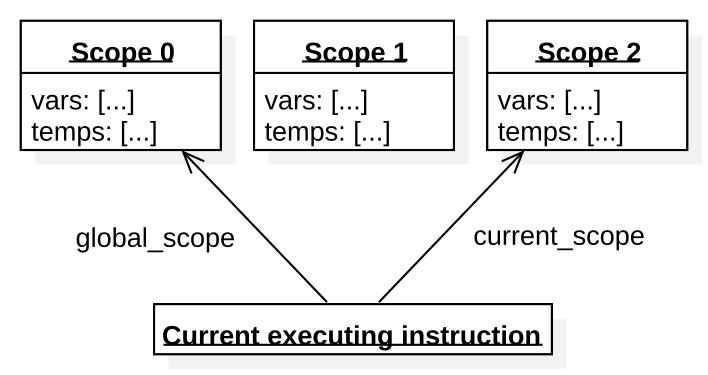
\includegraphics[width=220pt]{MemoryDiagram.png}
\end{figure}

During execution, the current instruction has access to two \texttt{Scope}s: the current scope, that is replaced every time a new scope is created and is accessed every time a local variable or a temporal value is read or written, and the global scope, accessed when a global variable is read or written. During execution of code in the global scope the reference to the current scope also points to the global scope, and local variables are mixed with global variables.

\section{\texttt{Value} enum}
This enum represents any type of value that can be used during runtime in \texttt{miniclj}. It is declared in file \path{miniclj-lib/src/vm/value.rs}.

\inputminted[firstline=16,lastline=30]{rust}{/home/mario/git/MarioJim/miniclj/miniclj-lib/src/vm/value.rs}

It has the following variants:
\begin{itemize}
  \item \texttt{Callable}, which stores a unique pointer to a structure that implements the trait \texttt{Callable}
  \item \texttt{Lambda}, which stores an instruction pointer and the arity of the function
  \item \texttt{List}, which stores a \texttt{List} value (explained in the next section)
  \item \texttt{Vector}, with a \texttt{Vec} of values inside
  \item \texttt{Set}, with a \texttt{HashSet} of values
  \item \texttt{Map}, with a \texttt{HashMap} of keys and values \texttt{Value}
  \item \texttt{String}
  \item \texttt{Number}, with a \texttt{Rational64} structure inside (a fraction of two 64-bit signed integers)
  \item \texttt{Nil}
\end{itemize}

\section{\texttt{List} enum}
This data structure is implemented as an enum with two variants, to closely match Clojure's implementation.

\inputminted[firstline=8,lastline=13]{rust}{/home/mario/git/MarioJim/miniclj/miniclj-lib/src/vm/list.rs}

Besides implementing a couple of useful functions like "nth" and "len", this enum implements two special functions: \texttt{from\_iter} which lets the virtual machine create a \texttt{List} from any iterator of \texttt{Value}s, and \texttt{try\_from}, which facilitates converting any type of value into a \texttt{List}. This last function only works for collections and strings, and for the other types it returns an error with the type of value passed (that couldn't be converted).

\inputminted[firstline=92,lastline=121]{rust}{/home/mario/git/MarioJim/miniclj/miniclj-lib/src/vm/list.rs}


\chapter{About callables}
The name "callable" was originally inherited by Clojure, where a callable refers to any value that can be called, or in other words, used as the first value in a s-expression. In this project, the name "callable" refers to any function exposed by the language or lambda functions defined by the user.

\section{Language callables and the \texttt{Callable} trait}
This type of callables implement the trait \texttt{Callable}, declared on file \path{miniclj-lib/src/callables/callable.rs}.

\inputminted[firstline=12,lastline=45,breaklines=true]{rust}{/home/mario/git/MarioJim/miniclj/miniclj-lib/src/callables/callable.rs}

A Rust trait shares the same idea as an abstract class in Java, but Rust structures don't actually "inherit" traits, they implement them, meaning polymorphism can't be used to downcast structures that implement the trait \texttt{Callable}, and that's why the language uses references to those callables through type \texttt{Box<dyn Callable>} (a \texttt{Box} is a unique pointer, and the keyword \texttt{dyn} means that they implement that trait).

On line 12, the \texttt{Callable} trait is declared, and for it to be implemented for a structure, the structure must also implement the traits \texttt{Display} (used to display values as strings, in the same spirit as \texttt{Object.toString()} in Java), \texttt{Debug} (also used to display structures as strings, but with more information) and \texttt{DynClone} (makes it easier to clone references to callables and to store them in \texttt{Box}es).

The \texttt{Callable} trait exposes 6 different functions, as seen in the code snippet above:
\begin{itemize}
  \item \texttt{name}, which returns a static reference to a string. This value is used when compiling code, to link a keyword (for example \texttt{defn}) to a callable (struct \texttt{Defn}, defined in file \texttt{scopefns.rs}).
  \item \texttt{compile}, receives a \texttt{CompilerState} structure and a vector of \texttt{SExpr}s as arguments, is the main function used during compilation to modify the state of the compiler. The default implementation calls the method \texttt{check\_arity} with the length of the vector of arguments and then calls \texttt{inner\_compile} with the state and the arguments.
  \item \texttt{check\_arity}, receives an unsigned integer and returns nothing, or a \texttt{CompilationError}. It doesn't have a default implementation.
  \item \texttt{inner\_compile}, accepts the same arguments as \texttt{compile}, and has a default implementation (used for language functions, language macros override this implementation), where it executes the following code:
  \begin{enumerate}
    \item First it calls the method \texttt{get\_as\_address} with the compiler state as the only argument. This function is used to include this function in the constants table of the \texttt{CompilerState}, and it returns a variant of the enum \texttt{Option<MemAddress>}: either \texttt{Some(address)} or \texttt{None}. The default implementation of this method returns \texttt{None}, and the \texttt{expect} call on the result of this method terminates the compiler with the included error message if the result is \texttt{None}. This forces any structures that implement \texttt{Callabe} to either implement \texttt{get\_as\_address} (for the callable to be used as a function) or override the default implementation of \texttt{inner\_compile} (for the callable to be used as a macro).
    \item Then, it converts the vector of \texttt{SExpr}s into an iterator, which is used to compile every s-expression into either a \texttt{MemAddress} or a \texttt{CompilationError}. These results are thenn collected into either a vector of \texttt{MemAdress}es or the first \texttt{CompilationError} that the compiler found. Finally, the question mark at the end of line 30 is an operator in Rust that makes it easier to handle errors: if the result of the iterator was a \texttt{CompilationError}, the whole function returns that \texttt{CompilationError}, and if the result of the iterator was the vector of \texttt{MemAddress}es, the function continues executing as normal.
    \item A new temporal address is created for the result of the function, and a new instruction is created to call the memory address of this function, with the memory addresses of its arguments, and lastly with the memory address where the function should save this result.
    \item Finally that instruction is inserted into the compiler and the temporal address used for the result is returned.
  \end{enumerate}
  \item \texttt{get\_as\_address}, as explained above, is used to insert this function in the constants table of the \texttt{CompilerState}, and it returns a variant of the enum \texttt{Option<MemAddress>}: either \texttt{Some(address)} or \texttt{None}.
  \item \texttt{execute}, this method is used during execution, and it receives the state of the virtual machine \texttt{VMState} and a vector of values. It returns a \texttt{RuntimeResult<Value>}: either a \texttt{Value} or a \texttt{RuntimeError}.
\end{itemize}

\subsection{Language functions}
Language functions are compiled with the process described above. An example of this type of callables is \texttt{IsEmpty}.

\inputminted[firstline=268,lastline=316]{rust}{/home/mario/git/MarioJim/miniclj/miniclj-lib/src/callables/collection/access.rs}

This function is used to test if a collection is empty or not, and is referenced in miniclj code by the symbol "empty?" (the string returned by the method \texttt{name}).

It overrides the method \texttt{check\_arity}, where it returns an error if the number of arguments passed to the function isn't equal to 1.

It also overrides \texttt{get\_as\_address} so that it returns a memory address asigned by the \texttt{CompilerState}, through calling its method \texttt{get\_callable\_address}.

Finally, it also provides an implementation for \texttt{execute}, where, first, the function, has to check for the number of arguments it received, because functions can be used as a value (for example, in transducers such as "filter").
  
Then, gets the first argument passed to it, and uses a match expression to check which type of argument it received. If it is a collection or a string, it checks if the underlying collection is empty; if it is "nil" it returns a true (because of a Clojure requirement), and if it is something else, the function returns a \texttt{RuntimeError}.

Line 316 calls a Rust macro, \texttt{display\_for\_callable}, defined in \path{minicl-lib/src/callables/mod.rs}, used to provide a default implementation of the \texttt{Display} trait (a trait used in Rust to represent a value as a string). This implementation uses the string provided in \texttt{Callable}'s method \texttt{name}.

\inputminted[lastline=9]{rust}{/home/mario/git/MarioJim/miniclj/miniclj-lib/src/callables/mod.rs}

\subsection{Language macros}
This callabes are separated into a different section because they have a different compilation process: they override \texttt{Callable}'s method \texttt{inner\_compile}, with the exception of callable \texttt{Recur}, which overrides the method \texttt{compile}.

The simplest example of this type of callables is \texttt{Do}, defined in \path{miniclj-lib/src/callables/groupingfns.rs}.

\inputminted[firstline=6,lastline=40,breaklines=true]{rust}{/home/mario/git/MarioJim/miniclj/miniclj-lib/src/callables/groupingfns.rs}

This macro is usually used to group calls to functions with side-effects. It receives any number of functions and returns only the result of the last one.

The overriden method \texttt{inner\_compile} does just that: it compiles the first s-expression, saves it's result address in variable \texttt{res\_addr}, and then iterates through the remaining s-expressions, compiling each one and replacing the variable \texttt{res\_addr} with the result of the compilation. After the iterator is exhausted, the variable \texttt{res\_addr} is returned.

Another important point is that every language macro overrides \texttt{execute} so that it automatically returns a \texttt{RuntimeError::CompilerError} (the variant of \texttt{RuntimeError} that indicates a bug in the compiler) with an error message detailing what happened and which function was called.

\subsection{\texttt{CallablesTable} struct}
This structure, defined in \path{miniclj-lib/src/callables/mod.rs}, stores a read-only map of callable names to pointers of callable structures. It is used both during compilation to compile macros and functions) and execution (to link callable names from the constants table to references to the corresponding structures).

\inputminted[firstline=47,lastline=48]{rust}{/home/mario/git/MarioJim/miniclj/miniclj-lib/src/callables/mod.rs}

It only has one method: a \texttt{get} method which receives a reference to a string and returns either a pointer to the callable with that name or nothing.

\inputminted[firstline=116,lastline=120]{rust}{/home/mario/git/MarioJim/miniclj/miniclj-lib/src/callables/mod.rs}

\section{User-defined functions}
Although there are three ways to write functions: using a "defn" call, using the "fn" macro, and using the shorthand syntax ("\#(...)"), all of them have a similar compilation and execution process.

\subsection{Compilation}
To exemplify the compilation process of these user-defined functions, here's the process for compiling a lambda defined using the shorthand syntax. It starts \texttt{CompilerState}'s main function: \texttt{compile}, which matches over the type of expression passed to it. Here's the actions executed when it encounters a lambda function defined with the shorthand syntax:

\inputminted[firstline=54,lastline=64,breaklines=true]{rust}{/home/mario/git/MarioJim/miniclj/miniclj-lib/src/compiler/state.rs}

First, a new inconditional jump instruction is created, with an unknown instruction pointer as a destination. This instruction is added to the compiler, and the index of this instruction is saved in variable \texttt{jump\_lambda\_instr\_ptr}. Then, the instruction pointer to the next instruction is saved, and a new constant is created using that pointer and the arity of the function, which for shorthand lambda functions is always 1. This constant is inserted into the compiler, and the address that corresponds to the lambda is saved in variable \texttt{lambda\_addr}.

The compiler then calls its own method \texttt{compile\_lambda} with the argument names (in shorthand lambdas it is only the symbol "\%") and the body of the function.

Finally, the jump in position \texttt{jump\_lambda\_instr\_ptr} is filled with the current instruction pointer, and the address of the lambda (\texttt{lambda\_addr}) is returned.

\texttt{compile\_lambda}, defined in the same file, executes a couple of actions:

\inputminted[firstline=86,lastline=105,breaklines=true]{rust}{/home/mario/git/MarioJim/miniclj/miniclj-lib/src/compiler/state.rs}

First, it creates a new \texttt{SymbolTable} structure using the shared pointer to the current, top-most \texttt{SymbolTable} and the number of arguments that the function receives. This last parameter is important because arguments in miniclj are treated as the first local variables in the \texttt{Scope} of the function, and if the user would like to create new local variables inside the function, these must have indexes greater than the index of the last parameter.

Then, the compiler iterates through the argument names, and inserts them in order to the \texttt{SymbolTable}. The compiler compiles the body of the function, and finally, destroys the created \texttt{SymbolTable}.

Lastly, \texttt{compile\_lambda} generates a return instruction using the returning address of compiling the body of the function, and appends it to the vector of instructions.

\subsection{Execution}
The execution of a user defined function starts when \texttt{VMState} tries to process a call instruction, where the address of the callable points to a \texttt{Lambda} value.

\inputminted[firstline=94,lastline=99,breaklines=true,autogobble]{rust}{/home/mario/git/MarioJim/miniclj/miniclj-lib/src/vm/state.rs}

In this case, the virtual machine calls its own function \texttt{execute\_lambda}, which receives the instruction pointer to jump to, the arity of the lambda function and the arguments passed to the function (as values). This function returns the value returned from the lambda, stores it in the parent scope of the function and advances the instruction pointer by 1.

\inputminted[firstline=40,lastline=66,breaklines=true,autogobble]{rust}{/home/mario/git/MarioJim/miniclj/miniclj-lib/src/vm/state.rs}

\texttt{execute\_lambda} is a simple function: it starts by comparing the number of arguments passed to the function and its arity, and if they aren't equal, the virtual machine returns a \texttt{RuntimeError::WrongArity} error.

Then, a new \texttt{Scope} structure is created, and the arguments passed to the function are inserted into it.

Finally, \texttt{VMState}'s method \texttt{inner\_execute} is called, which returns a \texttt{RuntimeResult<Option<MemAddress>>}. The error is handled by the question mark at the end of line 59, and we're left with either a memory address or nothing. In the first case, the value is extracted from the scope using the address, and it is returned by \texttt{execute\_lambda}. In the second case, \texttt{execute\_lambda} returns a \texttt{RuntimeError::CompilerError}, meaning the compiler has a bug and defined a lambda that never returned a value.


\chapter{Project structure}
The project is structured in 4 different folders; 3 Rust crates part of the root workspace, and one Next.js project:

\section{\texttt{miniclj-lib}}
This crate stores the main logic for the compiler, virtual machine and the shared code between them. This crate's unit tests are run for every new commit pushed to the main branch of the repo in a GitHub Actions worker, following the continuous integration pipeline described in the file \texttt{.github/workflows/ci.yml}.

This crate is divided in the following modules:
\begin{itemize}
  \item \texttt{callables}: Stores the callables available in the language, the base \texttt{Callable} trait, and the structure \texttt{CallablesTable} which exposes the callables implemented inside
  \item \texttt{compiler}: Stores the mechanisms and structures used specifically during the compilation process (the \texttt{CompilerState} struct, the \texttt{SymbolTable} enum, the \texttt{CompilationError} enum, the \texttt{SExpr} enum and the \texttt{Literal} enum)
  \item \texttt{constant}: Stores the implementation of the \texttt{Constant} enum
  \item \texttt{instruction}: Stores the implementation of the \texttt{Instruction} enum
  \item \texttt{memaddress}: Stores the implementation of the \texttt{MemAddress} struct
  \item \texttt{parsers}: Stores the parsers generated using \texttt{lalrpop} (the \texttt{SExprsParser}, \texttt{BytecodeParser} and the \texttt{NumberLiteralParser})
  \item \texttt{vm}: Stores the mechanisms and structures used specifically during the execution (the \texttt{VMState} struct, the \texttt{Scope} struct, the \texttt{RuntimeError} enum, the \texttt{Value} enum and the \texttt{List} enum)
\end{itemize}

\section{\texttt{miniclj}}
This crate stores only a couple of files; it exposes the compiler and vm functionality through a Command Line Interface. This crate compiles to an executable that can be called using the following subcommands for a different function each:
\begin{itemize}
  \item \texttt{check}: Check if a source code file can be correctly parsed
  \item \texttt{ast}: Print the abstract syntax tree from a source code file
  \item \texttt{build}: Compile a source code file into a bytecode file
  \item \texttt{exec}: Execute a bytecode file
  \item \texttt{run}: Compile and execute a source code file
\end{itemize}

\section{\texttt{miniclj-wasm}}
This crate compiles to a binary WebAssembly file, and exposes the functionality of the compiler and vm through JavaScript bindings so that they can be ran in a browser context. It exposes three functions, where each one accepts a string as the input code, and outputs either an structure with the output of the function or an error:
\begin{itemize}
  \item \texttt{ast}: This function prints the abstract syntax tree parsed from the code
  \item \texttt{compile}: This function compiles the code and outputs the corresponding bytecode
  \item \texttt{run}: This function compiles and executes the code, but with the following adaptations for the browser context:
  \begin{itemize}
    \item \texttt{read} calls are executed as \texttt{window.prompt} calls, where the browser displays an alert with a text input, which is then redirected to the program
    \item \texttt{print} and \texttt{println} instructions append its output to the global variable \\\texttt{window.minicljoutput}
  \end{itemize}
\end{itemize}

\section{\texttt{playground}}
This folder stores a simple, one page Next.js project where the \texttt{miniclj-wasm} is imported and executed for the code written in left side panel, and the output or the error for every function is displayed on the right side panel. The playground is built using GitHub Actions for each commit to the repo, following the continuous delivery pipeline described in the file \texttt{.github/workflows/cd.yml}


\chapter{Code examples}
\label{examples}

\section{Cyclic factorial function}
\subsection{\texttt{miniclj} code}
\inputminted{clojure}{/home/mario/git/MarioJim/miniclj/examples/cyclic_factorial.clj}

\subsection{Output}
\begin{minted}{text}
The factorial of 15 is 1307674368000
Finished in 26ms
\end{minted}

\subsection{Bytecode}
\inputminted{text}{/home/mario/git/MarioJim/miniclj/examples/cyclic_factorial.mclj}


\section{Recursive factorial function}
\subsection{\texttt{miniclj} code}
\inputminted{clojure}{/home/mario/git/MarioJim/miniclj/examples/recursive_factorial.clj}

\subsection{Output}
\begin{minted}{text}
The factorial of 15 is 1307674368000
Finished in 32ms
\end{minted}

\subsection{Bytecode}
\inputminted{text}{/home/mario/git/MarioJim/miniclj/examples/recursive_factorial.mclj}


\section{Factorial function using list generation and transducers}
\subsection{\texttt{miniclj} code}
\inputminted{clojure}{/home/mario/git/MarioJim/miniclj/examples/reduce_factorial.clj}

\subsection{Output}
\begin{minted}{text}
The factorial of 15 is 1307674368000
Finished in 12ms
\end{minted}

\subsection{Bytecode}
\inputminted{text}{/home/mario/git/MarioJim/miniclj/examples/reduce_factorial.mclj}


\section{Cyclic Fibonacci function}
\subsection{\texttt{miniclj} code}
\inputminted{clojure}{/home/mario/git/MarioJim/miniclj/examples/cyclic_fibonacci.clj}

\subsection{Output}
\begin{minted}{text}
The Fibonacci number 15 is 610
Finished in 27ms
\end{minted}

\subsection{Bytecode}
\inputminted{text}{/home/mario/git/MarioJim/miniclj/examples/cyclic_fibonacci.mclj}


\section{Recursive Fibonacci function}
\subsection{\texttt{miniclj} code}
\inputminted{clojure}{/home/mario/git/MarioJim/miniclj/examples/recursive_fibonacci.clj}

\subsection{Output}
\begin{minted}{text}
The Fibonacci number 15 is 610
Finished in 143ms
\end{minted}

\subsection{Bytecode}
\inputminted{text}{/home/mario/git/MarioJim/miniclj/examples/recursive_fibonacci.mclj}


\section{Find an element in a list}
\subsection{\texttt{miniclj} code}
\inputminted{clojure}{/home/mario/git/MarioJim/miniclj/examples/find_in_list.clj}

\subsection{Output}
\begin{minted}{text}
List: '(2 6 8 4 3 5)
Found element 3 in position 4
Finished in 26ms
\end{minted}

\subsection{Bytecode}
\inputminted{text}{/home/mario/git/MarioJim/miniclj/examples/find_in_list.mclj}


\section{Sorting a list}
\subsection{\texttt{miniclj} code}
\inputminted{clojure}{/home/mario/git/MarioJim/miniclj/examples/sort_list.clj}

\subsection{Output}
\begin{minted}{text}
List: (3 6 1 7 8 2 7)
Sorted list: (1 2 3 6 7 7 8)
Finished in 35ms
\end{minted}

\subsection{Bytecode}
\inputminted{text}{/home/mario/git/MarioJim/miniclj/examples/sort_list.mclj}


\section{Matrix multiplication}
\subsection{\texttt{miniclj} code}
\inputminted{clojure}{/home/mario/git/MarioJim/miniclj/examples/matrix_multiplication.clj}

\subsection{Output}
\begin{minted}{text}
Matrix A: ((3 6 7) (5 -3 0))
Matrix B: ((1 1) (2 1) (3 -3))
A x B: [[36 -12] [-1 2]]
B x A: [[8 3 7] [11 9 14] [-6 27 21]]
Finished in 18ms
\end{minted}

\subsection{Bytecode}
\inputminted{text}{/home/mario/git/MarioJim/miniclj/examples/matrix_multiplication.mclj}


\appendix

\definecolor{white}{rgb}{1,1,1}

\chapter{Commit log}
\label{apdx:commits}
\inputminted[bgcolor=white]{text}{/home/mario/git/MarioJim/miniclj/docs/commits.txt}

\chapter{Weekly logs in Spanish}
\label{apdx:weeklylogs}
\inputminted[bgcolor=white,breaklines=true]{md}{/home/mario/git/MarioJim/miniclj/docs/logs.md}

\chapter{lalrpop grammar}
\label{apdx:grammar}
\inputminted{rust}{/home/mario/git/MarioJim/miniclj/miniclj-lib/src/parsers/lispparser.lalrpop}


\end{document}
